\section{Project Description}
The project will focus on two different ways to play hockey. The first focus being traditional on-ice hockey, and the second focus being off-season dryland hockey. The on-ice hockey will be analyzed using ice hockey skates, whereas the off-season dryland hockey will be analyzed using rollerblades. Through observation of these two approaches, results will be taken according to how the participant shoots and skates. The various muscles that are involved in those activities will be recorded. These two different movements will then be compared to observe how well the dry land movements compare to one’s on ice movements. This will be completed using accelerometers to determine the speed and acceleration. Another apparatus that will be used are pressure sensors. These pressure sensors will be placed on the balls  and heels of the feet, which in turn will allow us to determine the amount of force that is applied when the skater uses their feet to push off of the ground and how their weight is being distributed during various actions. Finally, muscle sensors will be used to help determine which muscles are working during certain activities. The muscle sensors that will be used are EMG sensors. A conditioning circuit will need to be created in order to reduce the noise that the EMG sensors will create from the raw data. The conditions that will be in the circuit are for signal analysis.  Three main muscle groups will be focused on, the quadriceps, calves, and hamstrings. As displayed below in figure \ref{fig:front} and \ref{fig:back}, the muscles within the three muscle groups can be observed.
\begin{figure}[htbp]
\centering
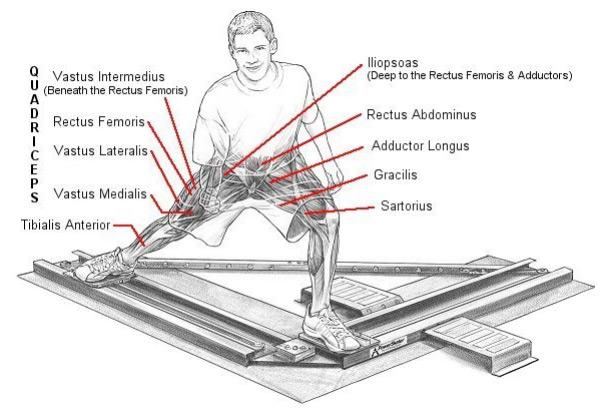
\includegraphics[scale=0.4]{Project_Proposal/figs/blog-muscles-used-for-skating-the-skating-anatomy-01.jpg}
\caption{The Anterior view of a Diagram of the Main Muscles that are 
used while Playing Hockey\cite{6}}
\label{fig:front}
\end{figure}

\begin{figure}[htbp]
\centering
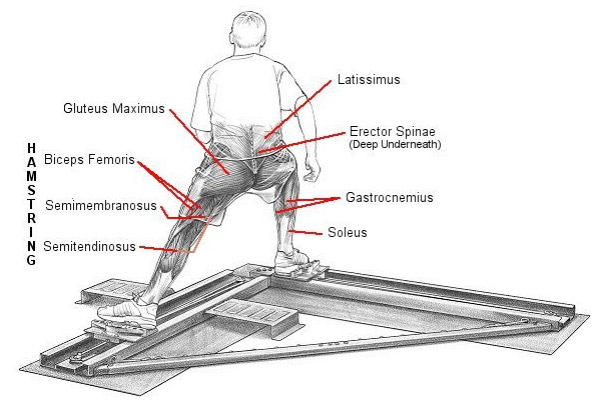
\includegraphics[scale =0.4]{Project_Proposal/figs/blog-muscles-used-for-skating-the-skating-anatomy-02.jpg}
\caption{The Posterior view of a Diagram of the Main Muscles that are 
used while Playing Hockey\cite{6}}
\label{fig:back}
\end{figure}

\par
Through experimentation of placement of the EMG sensors, the specific muscles within these groups will then be decided according to the most active. Each of the devices will be implemented using electrical circuits and the Arduino Uno microcontroller board. An electrical circuit will be constructed and will contain attachments to each of the instruments. There will be a separate circuit for each instrument, the accelerometer, pressure sensors, and the EMG muscle sensors. The data will be compared using the real experimental numbers, as well as compared using a Picoscope to observe the signal through a scope.
